 \documentclass{beamer}

\usetheme{MagdeburgFIN}
\usefonttheme{structurebold}
\usepackage{graphicx}
\usepackage{float}
\usepackage{url}
\usepackage{pdfpages}
\usepackage[export]{adjustbox}
\usepackage{wrapfig}
\usepackage{verbatim}

\title{MS-II. Concepts}
\author{Ali Hashaam, Ali Memon, Guzel Mussilova, Pavlo Shevchenko}
\date{May 23, 2017}
\institute{Scientific Project: Databases for Multi-Dimensional Data, Genomics and Modern Hardware}

\begin{document}

\begin{frame}[plain]
 \titlepage
\end{frame}

\begin{frame}
\frametitle{Table of Contents}
\tableofcontents 
\end{frame}

\section{Blinktopus}

\subsection{Octopus + BlinkDB = Blinktopus}

\begin{frame}
\frametitle{Octopus + BlinkDB = Blinktopus}
\begin{wrapfigure}{l}{1.6cm}
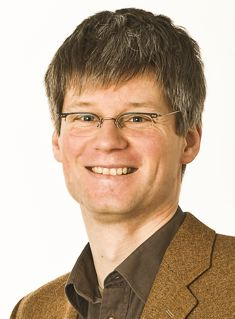
\includegraphics[width=1.65cm]{img/jensdittrich.jpg}
\vspace{0.25 cm}
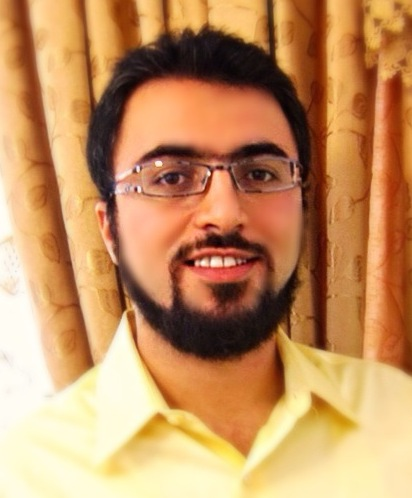
\includegraphics[width=1.75cm]{img/Mozafaribarzan.JPG}
\end{wrapfigure}
Create a new type of database system without fixed store that will mimic several existing systems\\
\vspace{2.2 cm}
The goal is to provide approximate answers with acceptable accuracy in orders of magnitude less time than that for the exact query processing.\footnote{\tiny Liu, Qing. Approximate Query Processing (Reference work entry) in: Liu, Ling, and M. Tamer Özsu. Encyclopedia of database systems. Vol. 6. Berlin, Heidelberg, Germany: Springer, 2009.}\\
\end{frame}

\subsection{Our Goal}
\begin{frame}
\frametitle{Our Goal}
To provide a \textbf{framework} that gives user a chance to act as \textit{Holistic SV Optimizer} like in OctopusDB \\
Add \textbf{Approximate Query Processing (AQP)} techniques\\
\textbf{Evaluate} performance depending on choice of SV
\end{frame}

\section{Concepts}

\begin{frame}
\frametitle{Octopus in Blinktopus}
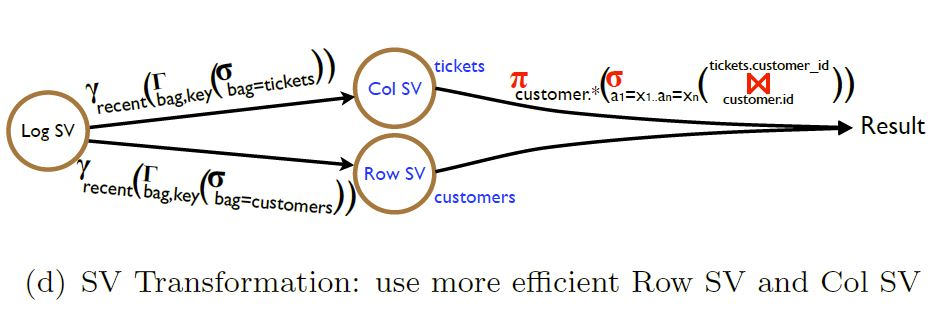
\includegraphics[scale=0.4]{img/SV_transformation.JPG}
\footnote{Jindal, Alekh. "OctopusDB: flexible and scalable storage management for arbitrary database engines." (2012).}
\end{frame}

\subsection{AQP.Architecture}
\begin{frame}
\frametitle{AQP.Architecture}
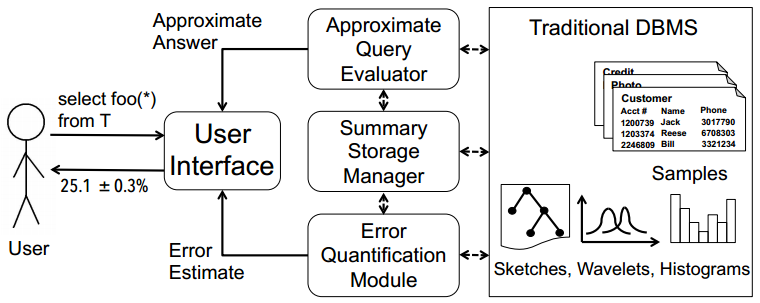
\includegraphics[scale=0.5]{img/blinkdb-workflow.png}
\footnote{The general anatomy of approximate query processing system}
\end{frame}

\begin{comment}

\subsection{AQP.User Interface}
\begin{frame}
\frametitle{AQP.User Interface}
Usually receives queries and accuracy or latency requirements from the user together with the approximate answers and the error bounds (or accuracy guarantees). \\
\vspace{0.3 cm}
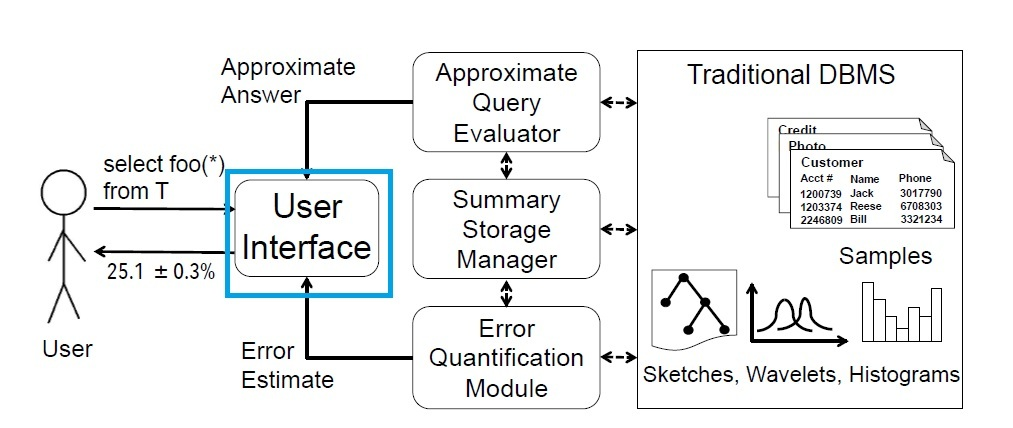
\includegraphics[scale=0.4]{img/aqp_ui.jpg}
%%\vspace{0.2 cm}
%%The majority of users are not statisticians, thus devising user-friendly and high-level mechanisms for expressing the error seems to be an area of research that requires more attention.
\end{frame}
\end{comment}

\subsection{AQP.Synopses Manager}
\begin{frame}
\frametitle{AQP.Synopses Manager}
A synopsis captures essential properties of the real data while taking less space.
\vspace{0.3 cm}
The synopses manager is responsible for:
\begin{itemize}
\item{Type of summary to use(Samples, histograms, sketches, wavelets etc.)}
\item{When to build it (offline vs. online)}
\item{How to store it (to use overlapping samples, how to structure/index/cache the synopses)}
\item{When to update it (batch or online)}
\end{itemize}
\end{frame}

\subsection{Types of Synopses}
\begin{frame}
\frametitle{Types of Synopses}
4 main families of synopses\footnote{\tiny Cormode, Graham, Minos Garofalakis, Peter J. Haas, and Chris Jermaine. "Synopses for massive data:
Samples, histograms, wavelets, sketches." Foundations and Trends in Databases 4, no. 1–3 (2012): 1-294.}:
\begin{itemize}
\vspace{0.3 cm}
\item{Samples}
\item{Histograms}
\item{Wavelets}
\item{Sketches}
\end{itemize}
\end{frame}

%%\subsection{Types of Synopses: Samples}
\begin{frame}
\frametitle{Types of Synopses: Samples}
Representative subset, chosen by stochastic sampling methods (e.g. Bernoulli, stratified,simple random with and without replacement).\pause
\vspace{0.2 cm}
\begin{itemize}
\item{Easy to implement.}
\item{Through adhering the same data structure as original tables support the widest range of queries.}
\item{Unbiased estimators for SUM/AVG queries are straightforwardly built.}
\item{Due to the immediate construction after issuing user query do not incur a delay.}
\item{Collecting more samples incrementally enhance imprecise estimates of a query results.}
\item{Without using the attribute value independence assumption allow high quality selectivity estimations.}
\end{itemize}
\end{frame}

%%\subsection{Types of Synopses: Samples}
\begin{frame}
\frametitle{Types of Synopses: Samples}
\begin{itemize}
\item{Poor estimations for less results.}
\item{Larger relations need more advanced techniques to make the sampling more scalable.}
\item{Selectivity estimations over larger datasets are less efficient.}
\item{Sensitive to skew and outliers.}
\item{Hard to use with (NOT-)/IN, DISTINCT, EXISTS queries.}
\item{Might be difficult to interpret by statistically unsophisticated users.}
\end{itemize}
\end{frame}

%%\subsection{Types of Synopses: Histograms}
\begin{frame}
\frametitle{Types of Synopses: Histograms}
A binned representation of the data distribution. The summary and bucket information is
used to (approximately) reconstruct the data in the bucket in order
to approximately answer the query.\pause
\vspace{0.2 cm}
\begin{itemize}
\item{A natural solution for range-sum queries.}
\item{Conceptual simplicity allows an effective use of a broad variety of estimation tasks(E.g. set-valued queries, real-valued data, and aggregate queries over predicates that more complex than simple ranges).}
\item{Relatively simple in interpretation.}
\item{Practically acceptable accuracies, provided that the “sufficient” storage space are allocated.}
\end{itemize}
\end{frame}

%%\subsection{Types of Synopses: Histograms}
\begin{frame}
\frametitle{Types of Synopses: Histograms}
\begin{itemize}
\item{Sensitive to dimensionality.}
\item{Performance strongly depends on bucketing schemes(how the buckets are chosen, what statistics are stored, how estimates are extracted, and what classes of query are supported).}
\item{Incremental maintenance.}
\item{Might provide too loose error estimates over the class of queries.}
\end{itemize}
\end{frame}

%%\subsection{Types of Synopses: Wavelets}
\begin{frame}
\frametitle{Types of Synopses: Wavelets}
Transform the data to represent significant features in a “frequency” domain and can capture combinations of high and low frequency information.\pause
\begin{itemize}
\item{Useful for range-sum queries.}
\item{Appropriately defined AQP algebra allows applying general SPJ (select, project, join) queries on relation summaries.}
\item{The linearity of the basic Haar transform manages a better maintenance under dynamic data than histograms.}
\item{Non-trivial to maintain wavelet coefficients under arbitrary update patterns.}
\item{Large number of coefficients must be retained to guarantee an accurate reconstruction of the data distribution in the multi-dimensional wavelet.}
\end{itemize}
\end{frame}

%%\subsection{Types of Synopses: Sketches}
\begin{frame}
\frametitle{Types of Synopses: Sketches}
\begin{itemize}
\item{Especially appropriate for streaming data.}
\item{Process fasters and easily paralleliazed if each new piece of data is independent of the current state of the summary.}
\item{Can be used as primitives within more complex mining operations, and to extract wavelet and histogram representations of streaming data.}
\end{itemize}
\end{frame}

%%\subsection{Types of Synopses: Sketches}
\begin{frame}
\frametitle{Types of Synopses: Sketches}
\begin{itemize}
\item{Mostly focused on answering a single type of query.}
\item{Number of parameters affects the accuracy and probability of failure.}
\item{Techniques do not extend well to more complex queries which combine multiple sub-queries.}
\item{The only complexity is mathematical (for complete accuracy estimation).}
\end{itemize}
\end{frame}

\begin{frame}
\frametitle{Types of Synopses: Sketches}
\begin{itemize}
\item{Transformation}
%%A transformation that gives the input data stream the property of white noise, or a uniform distribution of values. Input distinct keys are hashed and then the result is normalized to a uniform random value between zero and one.
\item{Data structure}
%%A data structure that follows a set of rules for retaining a small bounded set of the hash values. This fixed upper bound on sketch size enables straightforward memory management.
\item{Set of estimator algorithms}
%%A set of estimator algorithms that examines the sketch data structure and returns a result value.
\end{itemize}
\vspace{0.1cm}
The HyperLogLog is a famous sketch supporting count-distinct.
\begin{figure}
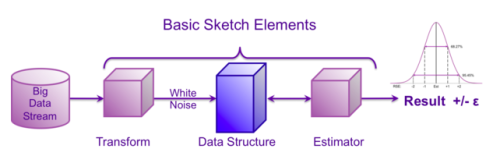
\includegraphics[scale=0.35]{img/distinct_count_sketches.png}
\caption{Distinct Count Sketch. High-level View.}
\end{figure}
\footnote{\tiny Source: https://yahooeng.tumblr.com/post/135390948446/data-sketches}
\end{frame}


\begin{comment}
%%\subsection{Types of Synopses: Others}
\begin{frame}
\frametitle{Types of Synopses: Others}
Other types of synopses given the specific queries:
\begin{itemize}
\vspace{0.25 cm}
\item{DISTINCT COUNT - HyperLogLog(HLL)}
\item{COUNT-GROUP BY - Count-Min-Sketch(CMS)}
\item{K-nearest neighbor - Neighbor Sensitive Hashing (KSH) tables}
\item{Foreign-key join - Join Synopsis}
\end{itemize}
\end{frame}
\end{comment}

\section{Building a Blinktopus}
\begin{frame}
\frametitle{Building a Blinktopus. Recall}
First, the Octopus:
\begin{itemize}
\item{Store incoming data in logs.}
\item{Query the logs (just a filter query).}
\item{Allow users to create views (row, column) over certain logs.}
\item{List all views and logs.}
\item{Launch the query over views or over logs, see the changes in performance.}
\end{itemize}
\end{frame}
\begin{frame}
\frametitle{Building a Blinktopus. Recall}
Enter AQP:
\begin{itemize}
\item{What synopsis can we easily support as a view for a specific query? Which will we choose to test? (Samples, histograms?)}
\item{Do Octopuses and AQP match well together?}
\item{How will we allow users to build this view?}
\item{How will we support queries using this view?}\\
\end{itemize}
\end{frame}


\begin{frame}
\frametitle{Building a Blinktopus. Workflow}
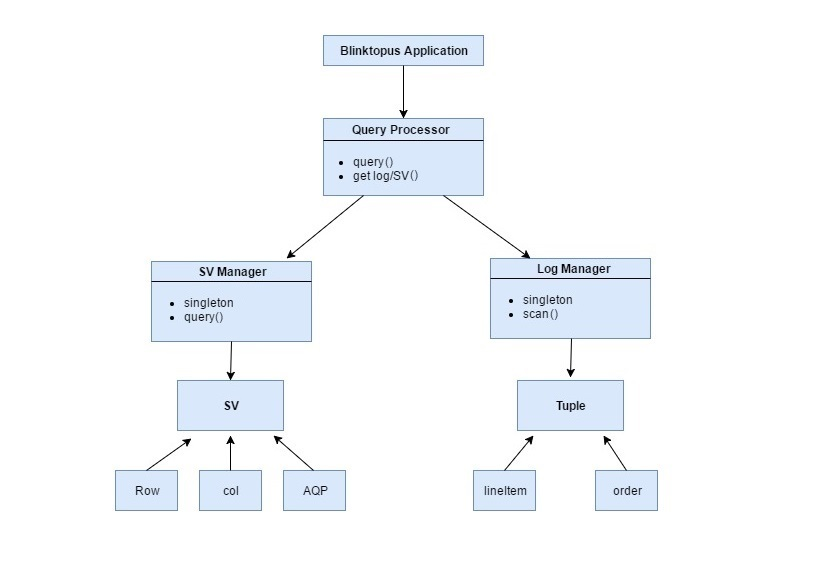
\includegraphics[scale=0.5]{img/workflow.jpg}
\end{frame}

%%\section{Building a Blinktopus. Progress}
\begin{frame}
\frametitle{Building a Blinktopus. IDE}
\begin{itemize}
\item{Back end}

\includegraphics[scale=0.3]{img/dropwizard.png}
\vspace{0.25 cm}
\item{Front end}

\includegraphics[scale=0.2]{img/jpnotebook.png}
\footnote{\tiny 
Sources: http://jupyter.org/\\
http://honstain.com/new-dropwizard-1-0-5-java-service/}
\end{itemize}
\end{frame}

\section{Project Organisation}

\subsection{Roles}
\begin{frame}
\frametitle{Project Organisation.Roles}
\textbf{Team:} \\
\hspace{0.3 cm}Guzel - Team Leader-Researcher\\
\hspace{0.3 cm}Pavlo - Developer\\
\hspace{0.3 cm}Ali H. - Developer\\
\hspace{0.3 cm}Ali M. - Researcher\\
\vspace{0.2 cm}
\textbf{Supervisor:} \\
\hspace{0.3 cm} Gabriel Campero Durand \\
\vspace{0.2 cm}
Changing roles after each milestone.
\\ \vspace{0.5 cm}
\textbf{Meetings:} \\ 
\hspace{0.5 cm} Team Meetings: Mo 14-15 \\
\hspace{0.5 cm} Meetings with supervisor: We 10-11
\end{frame}

\subsection{Schedule}
\begin{frame}
\frametitle{Project Organisation.Schedule}
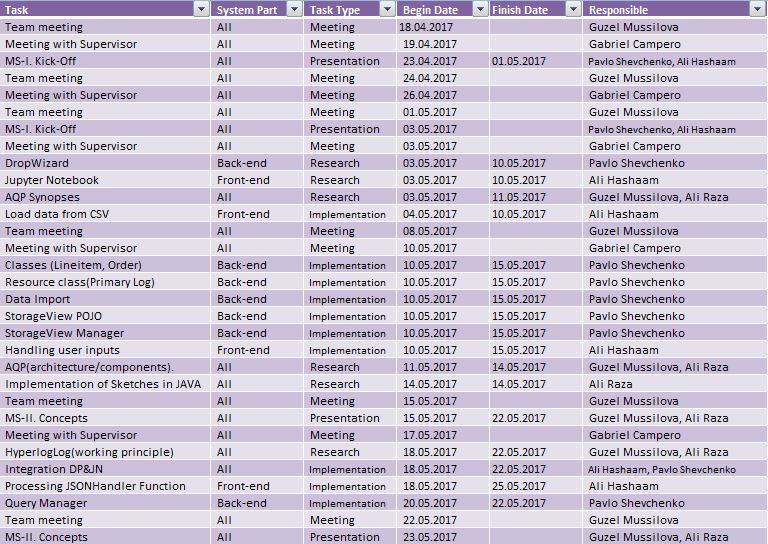
\includegraphics[scale=0.4]{img/Team_Schedule.jpg}
\end{frame}

\begin{frame}
 \frametitle{Thank you! Any questions?}
\end{frame}

\section{Literature}
\begin{frame}
\frametitle{Literature}
\begin{enumerate}
\item{Jindal, Alekh. "The mimicking octopus: Towards a one-size-fits-all database architecture." VLDB PhD Workshop. 2010.}
\item{Dittrich, Jens, and Alekh Jindal. "Towards a One Size Fits All Database Architecture." CIDR. 2011.}
\item{Jindal, Alekh. "OctopusDB: flexible and scalable storage management for arbitrary database engines." (2012).}
\item{Mozafari, Barzan. "Approximate query engines: Commercial challenges and research opportunities." SIGMOD, 2017.}
\item{Cormode, Graham, Minos Garofalakis, Peter J. Haas, and Chris Jermaine. "Synopses for massive data: Samples, histograms, wavelets, sketches." Foundations and Trends in Databases 4, no. 1–3 (2012): 1-294.}
\item{https://yahooeng.tumblr.com/post/135390948446/data-sketches}
\end{enumerate}
\end{frame}

\end{document}
